%%%%%%%%%%%%%%%%%%%%%%%%%%%%%%%%%%%%%%%%%%%%%%%%%
\section{Faire des animations}

%------------------------------------------------
\begin{frame}
  \frametitle{Pourquoi des animations ?}
  
  \begin{itemize}
   \flch Faire des animations sur une diapositive permet que son contenu arrive progressivement, de manière synchrone avec votre discours.
  Cela évite que votre public lise une formule compliquée encadrée en fin de diaopositive au lieu de vous écouter expliquer le début de la diapositive.\\
  \flch Dans le cas où vous avez fait une simulation dynamique, cela permet de simuler un petit dessin animé dans un fichier pdf autorisé aux concours.
  \end{itemize}
\end{frame}

%++++++++++++++++++++++++++++++++++++++++++++++++
\subsection{Sur une diapo quelconque}
%------------------------------------------------
%\begin{frame}
%	\frametitle{Suite d'équations animée avec \lin{\pause}}
%	On reprend la suite d'équations présentée plus haut, mais grâce à des commandes \lin{\pause}, celles-ci apparaissent au fur et à mesure.
%	\begin{align*}
%	  \pause
%		a \pause
%		& = b+c+d * \sum_{i=1}^n x_i \pause \\
%		& = b+c+d * \sum_{i=1}^n (z_i - y_i) \pause \\
%		& \leqslant B+c+d * \sum_{i=1}^n (z_i - y_i) & \pause
%		\textcolor{expli}{\textit{ ici une petite explication}}\\
%	\end{align*}
%\end{frame}


%------------------------------------------------
\begin{frame}
	\frametitle{Formules au fur et à mesure avec \lin{\pause}}
	On reprend la suite d'équations présentée plus haut, mais grâce à des commandes \lin{\pause}, celles-ci apparaissent au fur et à mesure.
	\pause
	Voilà une formule juste centrée car entre \lin{$$} et \lin{$$} 
	$$ A  = \sum_{i=1}^{n} a_i +b_i$$
	
	\pause
	Voilà une formule encadrée avec \lin{\fbox}et centrée 
	\begin{center}
		\fbox{$\Delta^{early}_u\!(E,\!T) \!\geqslant 0$ if $u \in E$}
	\end{center}
	\pause
	
	Voilà une formule encadrée en couleurs avec \lin{\fcolorbox} et centrée
	\begin{center}
		\fcolorbox{turquoiseFonce}{white}{$\Delta^{early}_u\!(E,\!T) \!\geqslant 0$ if $u \in E$}
	\end{center}
\end{frame}

%------------------------------------------------
\begin{frame}
  \frametitle{Exemple avec \lin{\only}}

  \only<1>{N'apparaît que sur la slide "1", grâce à \lin{\only<1>{...}},\\
  puis disparaît et laisse sa place.\\
  }
  \couleur { partie là tout le temps}, car hors d'un \texttt{$\backslash$only<1>}\\

  \only<2-4>{N'apparaît que sur les slides "2", "3" et "4",
  grâce à \texttt{$\backslash$only<2-4>\{...\}},\\
  puis disparaît et laisse sa place.\\
  }

  \only<2>{N'apparaît que sur la slide "2", grâce à \texttt{$\backslash$only<2>\{...\}},\\
  puis disparaît et laisse sa place.\\
  }

  \only<3->{Apparaît de la slide "3" à la fin, grâce à \texttt{$\backslash$only<3->\{...\}}, avant sa place n'est pas reversée
  }
\end{frame}


%------------------------------------------------
\begin{frame}
\frametitle{Exemple avec \lin{\onslide}}

\onslide<1>{N'apparaît que sur la slide "1", grâce à \texttt{$\backslash$onslide<1>\{...\}},\\
mais ici sa place est reversée, pas réutilisée.\\
}
\couleur { partie là tout le temps}, car hors d'un \texttt{$\backslash$onslide<1>}\\

\onslide<2-4>{N'apparaît que sur les slides "2", "3" et "4",
grâce à \texttt{$\backslash$only<2-4>\{...\}},\\
mais ici sa place est reversée, pas réutilisée.\\
}

\onslide<2>{N'apparaît que sur la slide "2", grâce à \texttt{$\backslash$onslide<2>\{...\}},\\
mais ici sa place est reversée, pas réutilisée.\\
}

\onslide<3->{Apparaît de la slide "3" à la fin, grâce à \texttt{$\backslash$onslide<3->\{...\}},
mais sa place est reversée, pas réutilisée.\\
}
\end{frame}



%++++++++++++++++++++++++++++++++++++++++++++++++
\subsection{Avec des images}
%------------------------------------------------
\begin{frame}
\frametitle{Images animées - exemple - le début à la main}
  \begin{figure}
	  \only<1>{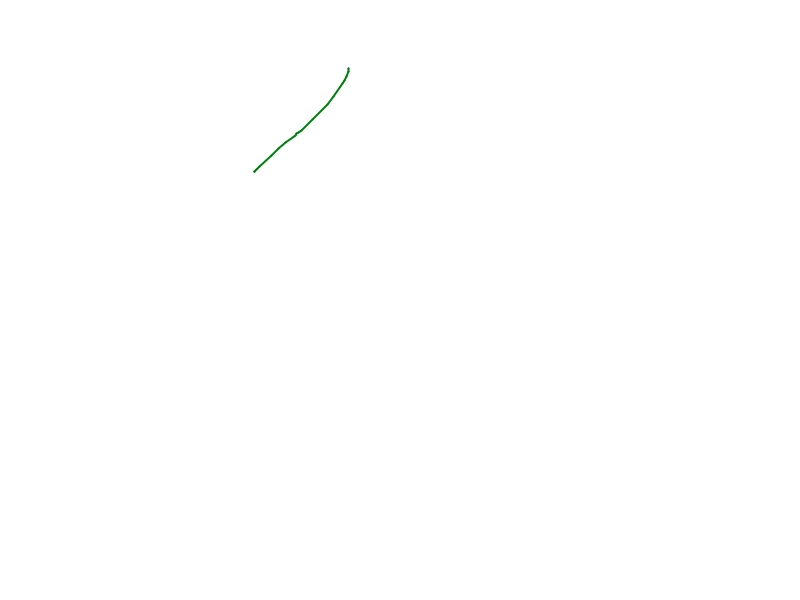
\includegraphics[scale=0.45]{pour_exemples/anim/img1.jpg}}
	  \only<2>{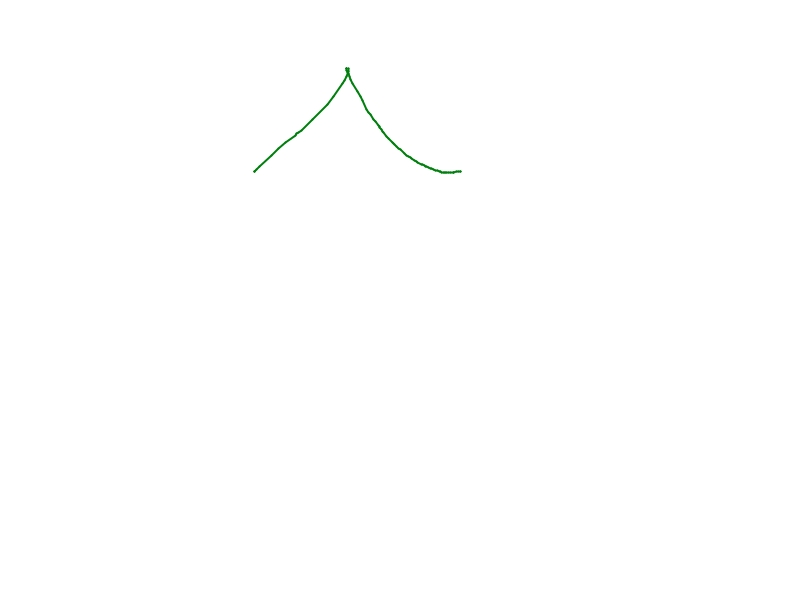
\includegraphics[scale=0.45]{pour_exemples/anim/img2.jpg}}
	  \only<3>{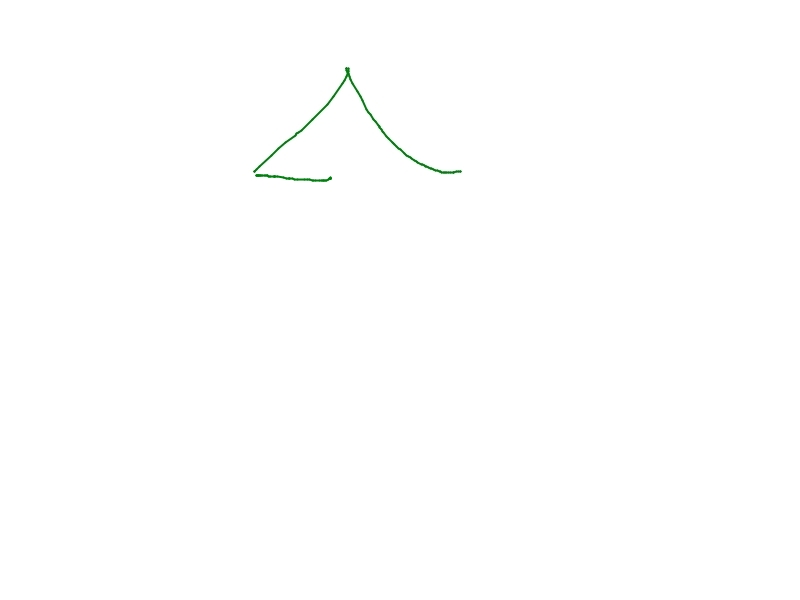
\includegraphics[scale=0.45]{pour_exemples/anim/img3.jpg}}
%	  \only<4>{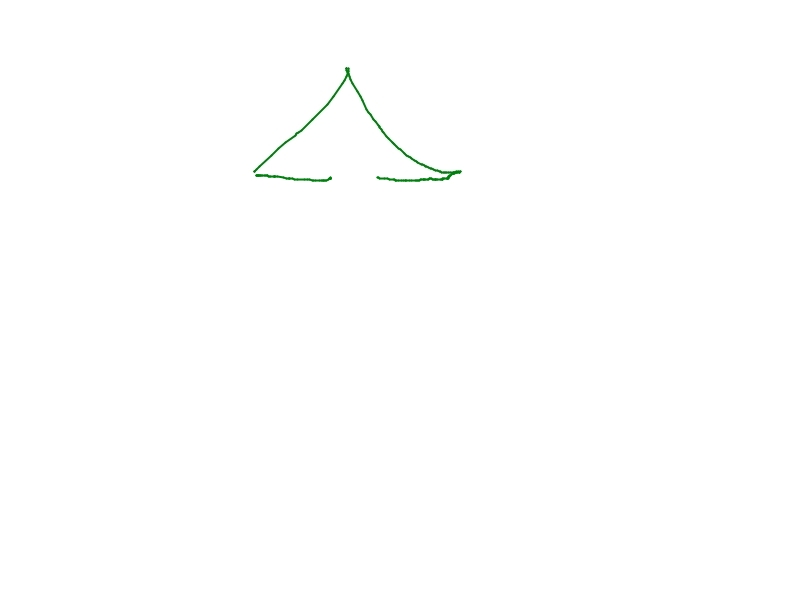
\includegraphics[scale=0.45]{pour_exemples/anim/img4.jpg}}
%	  \only<5>{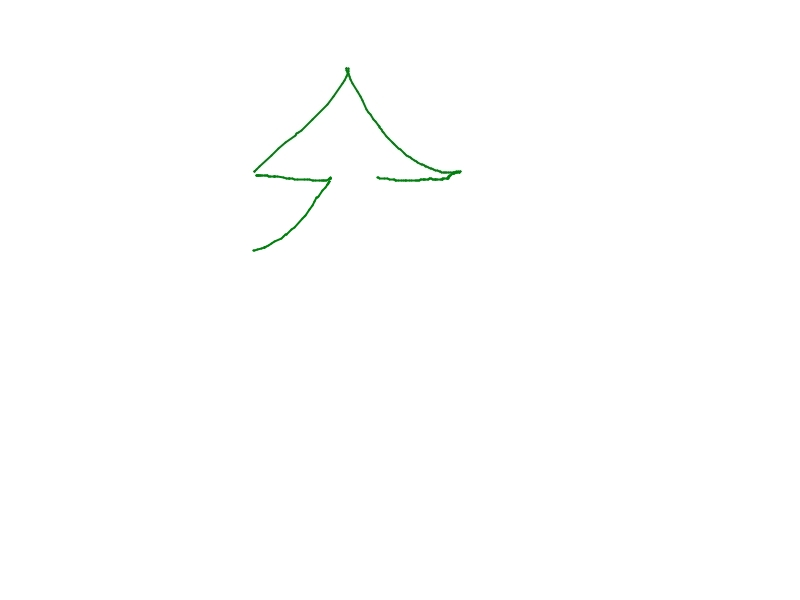
\includegraphics[scale=0.45]{pour_exemples/anim/img5.jpg}}
%	  \only<6>{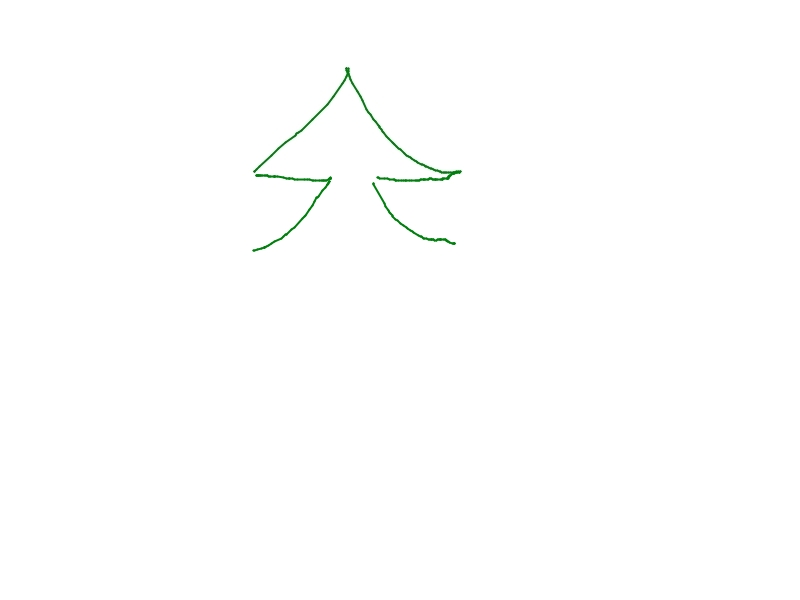
\includegraphics[scale=0.45]{pour_exemples/anim/img6.jpg}}
%	  \only<7>{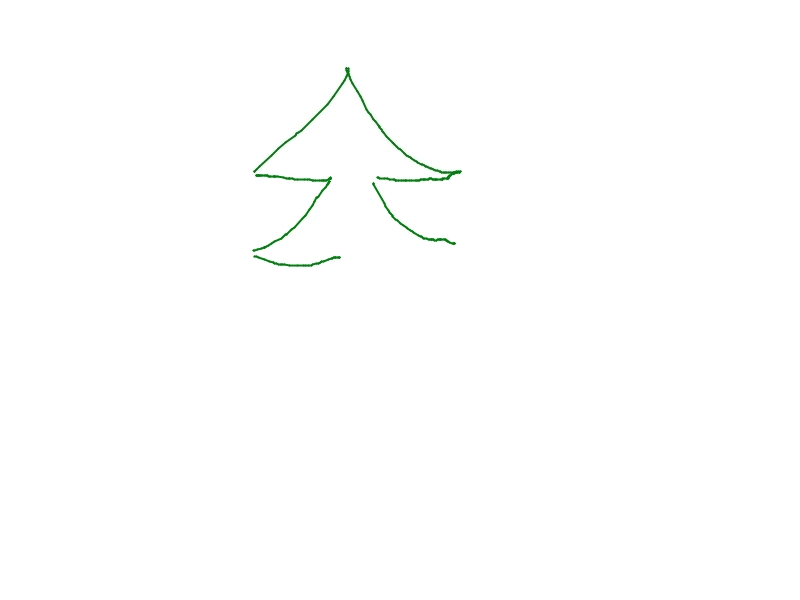
\includegraphics[scale=0.45]{pour_exemples/anim/img7.jpg}}
%	  \only<8>{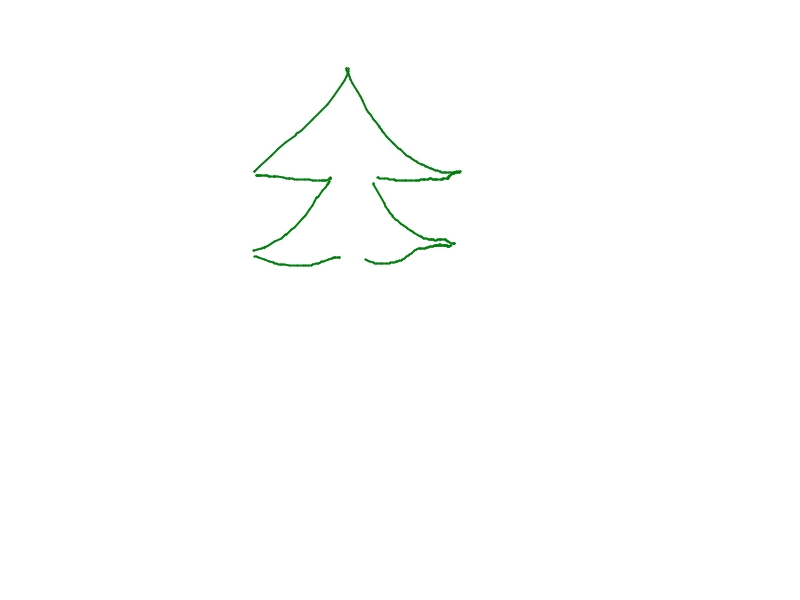
\includegraphics[scale=0.45]{pour_exemples/anim/img8.jpg}}
%	  \only<9>{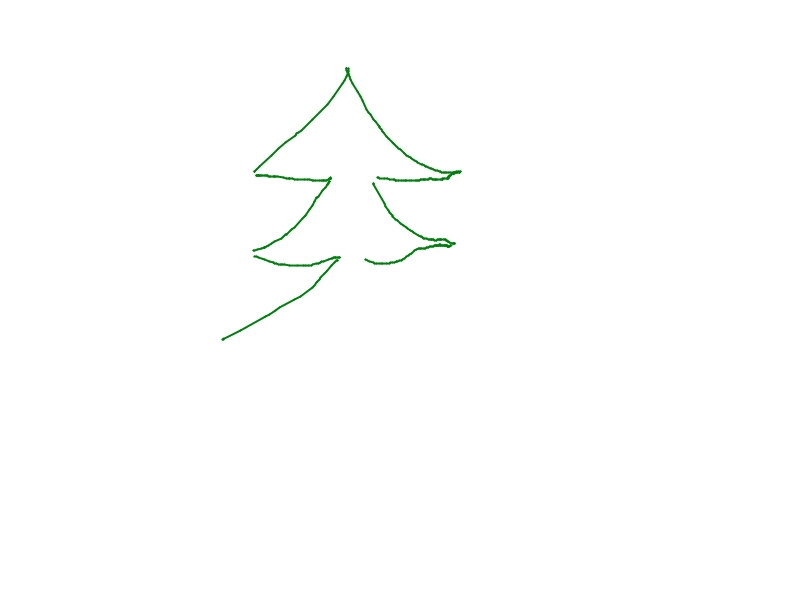
\includegraphics[scale=0.45]{pour_exemples/anim/img9.jpg}}
%	  \only<10>{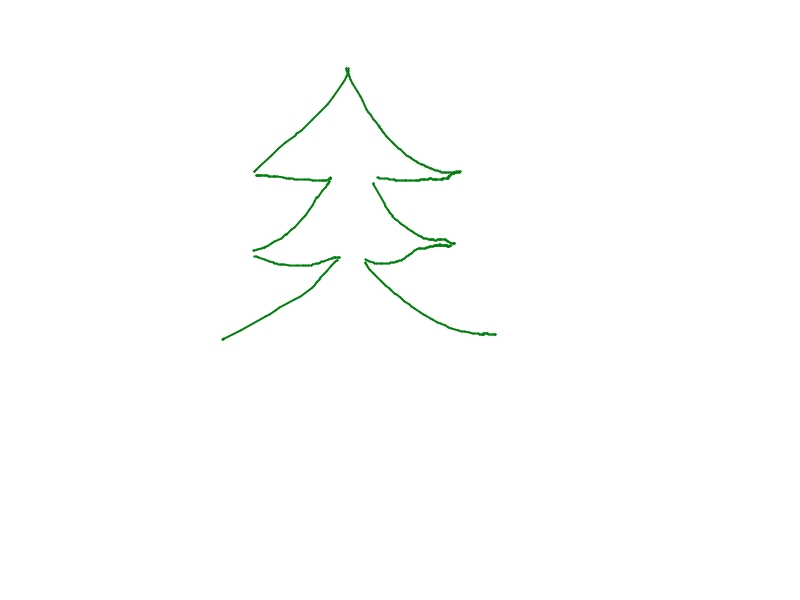
\includegraphics[scale=0.45]{pour_exemples/anim/img10.jpg}}
%	  \only<11>{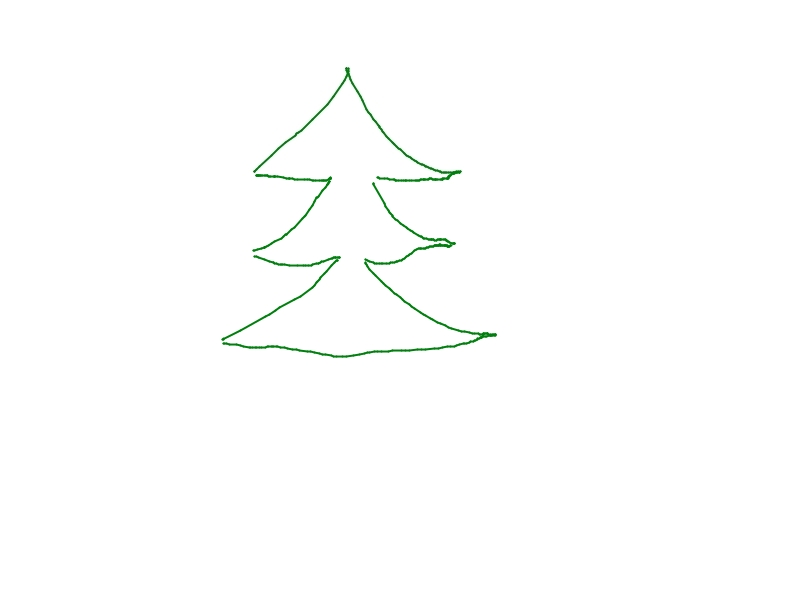
\includegraphics[scale=0.45]{pour_exemples/anim/img11.jpg}}
  \end{figure}
\end{frame}

%------------------------------------------------
\begin{frame}
  \frametitle{Images animées - exemple - le tout avec \lin{\foreach}}
  \begin{figure}
    \foreach \k in{1,2,...,11}{
	    \only<\k>{
	      {Image \k}
	      \includegraphics[scale=0.45]{pour_exemples/anim/img\k.jpg}
	    }
	  }
  \end{figure}
\end{frame}

%------------------------------------------------
\begin{frame}
  \frametitle{Images animées - explications}
  
  \begin{itemize}
    \flch On nomme les images à afficher successivement avec des noms comme \texttt{im1.jpg}, \texttt{im2.jpg}...
    où la numérotation suit bien sûr l'ordre dans lequel doivent apparaître ces images.
    \flch On peut alors faire des copier-coller de \lin{inludegraphics{im1.jpg}} en vhangeant le numéro, ou bien utiliser \lin{\foreach} pour faire une boucle
    \flch Attention le poids du PDF de présentation augmente très vite, or vous êtes limités en taille pour le PDF à envoyer aux concours (à 5Mo je crois).
    Vous pouvez commenter la slide qui inclut les 11 images du sapin, recompiler,  et observer que la taille du PDF a réduit d'un volume équivalent à la somme des 11 images (un peu plus même).
    Donc il faut avoir peu d'images (pas 50) ou des petites images, ou bien se mettre au tikz...
  \end{itemize}
\end{frame}




%++++++++++++++++++++++++++++++++++++++++++++++++
\subsection{Avec du tikz}
%------------------------------------------------
\begin{frame} [fragile]
  \frametitle{Exemple avec tikZ - v1}*
  
  On peut utiliser  \texttt{$\backslash$draw<n->} pour animer directement
  une figure tikz.\\[0.2cm]
  \alert{Attention}, la figure est replacée automatiquement à chaque étape en fonction de la place occupée par la figure à cette étape, donc si on veut voir le point bouger dans l'exemple ci-dessous, il faut un cadre fixe
  \begin{center}
    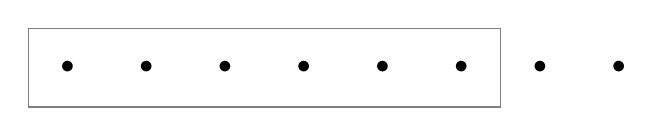
\begin{tikzpicture} 
    %cadre
    \draw[gray](0.5,-0.5)rectangle(6.5,0.5);
    %points
    \foreach \step in {1,2,3,...,8} {
      \draw<\step>(\step,0) node{$\bullet$};
    }
    \end{tikzpicture}
  \end{center}

\end{frame}

%------------------------------------------------
\begin{frame} [fragile]
  \frametitle{Exemple avec tikZ - v1}
  
  De plus, cet ajustement automatique rend parfois les animations désagréables,
  comme juste avant les deux derniers points qui ont tout fait bouger.
  Il faut donc mettre un cadre qui englobe la superposition de toutes les étapes.
  Exemple ci-dessous :
  \begin{center}
    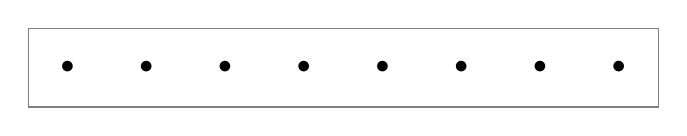
\begin{tikzpicture} 
      %cadre
      \draw[gray](0.5,-0.5)rectangle(8.5,0.5);
      %points
      \foreach \step in {1,2,3,...,8} {
        \draw<\step>(\step,0) node{$\bullet$};
      }
    \end{tikzpicture}
  \end{center}

\end{frame}



%++++++++++++++++++++++++++++++++++++++++++++++++
\subsection{Animation et numérotation}
%------------------------------------------------
\begin{frame}
\frametitle{Animation et numérotation\esp}
	Comme on peut le voir sur les slides précédentes, il y a par défaut un seul numéro pour les différents slides issues des animations d'une seule "frame". 
	Autrement dit on a un numéro de slide pour chaque occurence d'un environnement \lin{frame}.
	\medskip
	
	Dans la plupart des cas ce comportement par défaut est opportun, mais dans le cas où l'on veut pouvoir faire référence à une étape précise de l'animation, comme dans un déroulé d'algorithme par exemple, on peut ajouter des numéros.
	Pour cela, on incrémente \textit{manuellement} le compteur \texttt{framenumber} grâce à la commande \lin{\addtocounter{framenumber}{1}}.
\end{frame}

%------------------------------------------------
\addtocounter{framenumber}{-1}
\begin{frame}
\frametitle{Numéroter chaque étape d'une animation avec \lin{\pause}}
 	\addtocounter{framenumber}{1}
	Si on utilise des \lin{\pause}, il suffit de mettre une seule fois l'incrémentation \lin{\addtocounter{framenumber}{1}} juste après le \lin{\begin{frame}} car elle est ré-évaluée pour chaque slide.
	Comme elle est évaluée la première fois alors que le \lin{\begin{frame}} incrémente déjà automatiquement ce compteur, on compense en décrémentant avant le \lin{\begin{frame}}.
	\medskip
	Exemple ici  : 
	\begin{itemize}
		\item étape 1 \pause
		\item étape 2 \pause
		\item étape 3 \pause
	\end{itemize}
	
\end{frame}

%------------------------------------------------
\addtocounter{framenumber}{-1}
\begin{frame}
\frametitle{Numéroter chaque étape d'une animation avec \lin{\only}}
 	\addtocounter{framenumber}{1}
 	Avec des  \lin{\only} ça marche pareil : il suffit de mettre une seule fois \lin{\addtocounter{framenumber}{1}} juste après le \lin{\begin{frame}} et une seule fois \lin{\addtocounter{framenumber}{-1}} juste avant.
	\medskip
	Exemple ici : 
	\begin{itemize}
		\only<1>{\item étape 1}
		\only<2->{\item étape 2 et suivantes}
		\only<3>{\item étape 3}
	\end{itemize}
\end{frame}
